\documentclass[border=1pt]{standalone}
% Shared preamble for the PixelRoot figures: Times text and math to match
% IEEEtran; every figure is drawn at its printed size (no scaling in the paper).
\usepackage[T1]{fontenc}
\usepackage{mathptmx}
\usepackage{amsmath}
\usepackage{xcolor}
\usepackage{tikz}
\usetikzlibrary{arrows.meta,positioning,calc,fit,backgrounds,decorations.pathreplacing,shapes.geometric}
\definecolor{ink}{HTML}{1B2838}
\definecolor{acc}{HTML}{1F5FBF}
\definecolor{grn}{HTML}{1E7B3A}
\definecolor{red}{HTML}{B3261E}
\definecolor{amb}{HTML}{9A6B00}
\definecolor{cu}{HTML}{B87333}
\tikzset{
  >={Stealth[length=1.6mm,width=1.2mm]},
  every picture/.style={line width=0.6pt, font=\footnotesize, color=ink},
  blk/.style={draw=ink, rounded corners=1.5pt, align=center, inner sep=2.5pt,
    minimum height=9mm, fill=white},
  note/.style={font=\scriptsize, align=left, text=ink!80},
}

\begin{document}
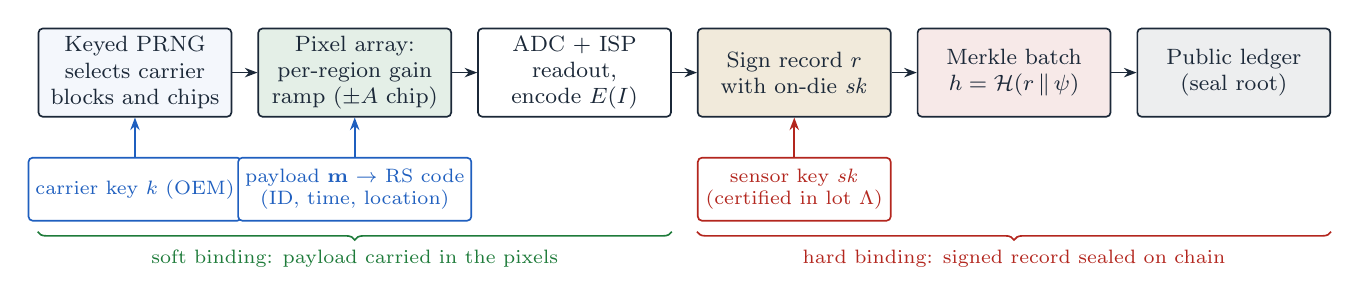
\begin{tikzpicture}[node distance=3.2mm]
\tikzset{b/.style={blk, minimum width=2.45cm, minimum height=1.12cm, fill=#1},
         inp/.style={blk, minimum width=2.45cm, minimum height=0.8cm, draw=#1, text=#1, font=\scriptsize}}
\node[b=acc!5] (prng) {Keyed PRNG\\selects carrier\\blocks and chips};
\node[b=grn!12, right=of prng] (mod) {Pixel array:\\per-region gain\\ramp ($\pm A$ chip)};
\node[b=white, right=of mod] (adc) {ADC + ISP\\readout,\\encode $E(I)$};
\node[b=amb!14, right=of adc] (sign) {Sign record $r$\\with on-die $\mathit{sk}$};
\node[b=red!10, right=of sign] (merk) {Merkle batch\\$h=\mathcal{H}(r\,\|\,\psi)$};
\node[b=ink!8, right=of merk] (led) {Public ledger\\(seal root)};
\foreach \a/\b in {prng/mod, mod/adc, adc/sign, sign/merk, merk/led} \draw[->] (\a) -- (\b);
\node[inp=acc, below=5mm of prng] (k) {carrier key $k$ (OEM)};
\node[inp=acc, below=5mm of mod] (m) {payload $\mathbf{m}$ $\to$ RS code\\(ID, time, location)};
\node[inp=red, below=5mm of sign] (sk) {sensor key $\mathit{sk}$\\(certified in lot $\Lambda$)};
\draw[->, acc] (k) -- (prng);
\draw[->, acc] (m) -- (mod);
\draw[->, red] (sk) -- (sign);
% binding brackets
\draw[decorate, decoration={brace, amplitude=3pt, mirror}, grn] ($(prng.south west)+(0,-1.45)$) -- node[below=3pt, font=\scriptsize, text=grn] {soft binding: payload carried in the pixels} ($(adc.south east)+(0,-1.45)$);
\draw[decorate, decoration={brace, amplitude=3pt, mirror}, red] ($(sign.south west)+(0,-1.45)$) -- node[below=3pt, font=\scriptsize, text=red] {hard binding: signed record sealed on chain} ($(led.south east)+(0,-1.45)$);
\end{tikzpicture}
\end{document}
